\documentclass[11pt,a4paper]{article}
\usepackage[margin=1in]{geometry}
\usepackage[T1]{fontenc}
\usepackage[utf8]{inputenc}
\usepackage{lmodern}
\usepackage{microtype}
\usepackage{amsmath,amssymb}
\usepackage{booktabs}
\usepackage{siunitx}
\usepackage{hyperref}
\usepackage{xcolor}
\usepackage{graphicx}
\usepackage{tikz}
\usetikzlibrary{arrows.meta,positioning,shapes.geometric,fit}

\hypersetup{
  colorlinks=true,
  linkcolor=blue,
  urlcolor=blue,
  pdftitle={Team MindMatrix - Final Technical Report},
  pdfauthor={Team MindMatrix}
}

\title{\textbf{Team MindMatrix Final Technical Report}\\
\large Autonomous Constellation Manager for Space Debris Risk Mitigation}
\author{Team MindMatrix}
\date{April 2026}

\begin{document}
\maketitle

\begin{abstract}
This report presents the final submission architecture and methods implemented by Team MindMatrix for autonomous conjunction monitoring and maneuver planning in low Earth orbit operations. The solution integrates physically grounded orbital propagation, efficient spatial screening, constrained maneuver optimization, and an interactive operations dashboard. We provide equations for the numerical methods, algorithmic details for risk detection and optimization, and system-level design diagrams for end-to-end execution.
\end{abstract}

\section{Problem and Objectives}
The system is designed to continuously monitor a constellation, predict close approaches with debris, and trigger safe maneuvers under fuel and operations constraints. The practical objectives are:
\begin{enumerate}
  \item maintain real-time situational awareness,
  \item detect conjunctions at scale,
  \item minimize collision risk while preserving mission continuity,
  \item provide transparent operator controls and telemetry.
\end{enumerate}

\section{Numerical Methods}
\subsection{State Dynamics}
Each orbiting object is modeled with ECI state vector
\[
\mathbf{x} = [x,y,z,v_x,v_y,v_z]^T.
\]
The propagation model combines two-body gravity with J2 perturbation:
\[
\dot{\mathbf{r}} = \mathbf{v}, \qquad
\dot{\mathbf{v}} = -\mu\frac{\mathbf{r}}{\|\mathbf{r}\|^3} + \mathbf{a}_{J2}.
\]
The J2 acceleration is
\[
\mathbf{a}_{J2}=\frac{3J_2\mu R_E^2}{2\|\mathbf{r}\|^5}
\begin{bmatrix}
x\left(5\frac{z^2}{\|\mathbf{r}\|^2}-1\right)\\
y\left(5\frac{z^2}{\|\mathbf{r}\|^2}-1\right)\\
z\left(5\frac{z^2}{\|\mathbf{r}\|^2}-3\right)
\end{bmatrix}.
\]

\subsection{Time Integration}
A fixed-step RK4 method is used:
\begin{align*}
\mathbf{k}_1 &= f(\mathbf{x}_n), \\
\mathbf{k}_2 &= f\left(\mathbf{x}_n + \frac{\Delta t}{2}\mathbf{k}_1\right), \\
\mathbf{k}_3 &= f\left(\mathbf{x}_n + \frac{\Delta t}{2}\mathbf{k}_2\right), \\
\mathbf{k}_4 &= f\left(\mathbf{x}_n + \Delta t\mathbf{k}_3\right), \\
\mathbf{x}_{n+1} &= \mathbf{x}_n + \frac{\Delta t}{6}(\mathbf{k}_1 + 2\mathbf{k}_2 + 2\mathbf{k}_3 + \mathbf{k}_4).
\end{align*}
Operationally, long user-requested steps are chunked to keep API responsiveness stable.

\subsection{Initialization}
Initial states are produced from TLE catalogs via SGP4 at epoch $t_0$:
\[
(\mathbf{r}_0,\mathbf{v}_0)=\mathrm{SGP4}(\mathrm{TLE},t_0).
\]

\section{Spatial Optimization and Risk Algorithms}
\subsection{KD-Tree Candidate Screening}
Brute-force pair search is avoided by KD-tree broad-phase filtering. For satellites set $\mathcal{S}$ and debris set $\mathcal{D}$ at time step $t_k$:
\[
\mathcal{C}_k = \left\{(i,j)\in\mathcal{S}\times\mathcal{D}:\|\mathbf{r}_i(t_k)-\mathbf{r}_j(t_k)\|\le r_{\mathrm{screen}}\right\}.
\]
This reduces screening from all-pairs complexity toward practical near-neighbor search.

\subsection{Collision Probability Approximation}
For short encounters, collision probability uses a Chan-style approximation:
\[
P_c \approx \frac{R^2}{2\sigma^2}\exp\left(-\frac{d^2}{2\sigma^2}\right),
\]
where $d$ is miss distance, $R$ is hard-body radius, and $\sigma$ is position uncertainty scale.

\subsection{Maneuver Optimization Under Constraints}
Fuel update follows Tsiolkovsky:
\[
\Delta m = m_0\left(1-\exp\left(-\frac{\Delta v}{I_{sp}g_0}\right)\right).
\]
A practical planning score is
\[
J = w_1\Delta d_{\min} - w_2\|\Delta\mathbf{v}\| - w_3\Delta m - w_4\tau_{\mathrm{outage}},
\]
subject to
\begin{align*}
\|\Delta\mathbf{v}\| &\le \Delta v_{\max}, \\
t_{k+1}^{\mathrm{burn}}-t_k^{\mathrm{burn}} &\ge t_{\mathrm{cooldown}}, \\
m_{\mathrm{fuel}}-\Delta m &\ge 0.
\end{align*}

\section{System Architecture}
\subsection{Layered Design}
\begin{figure}[h!]
\centering
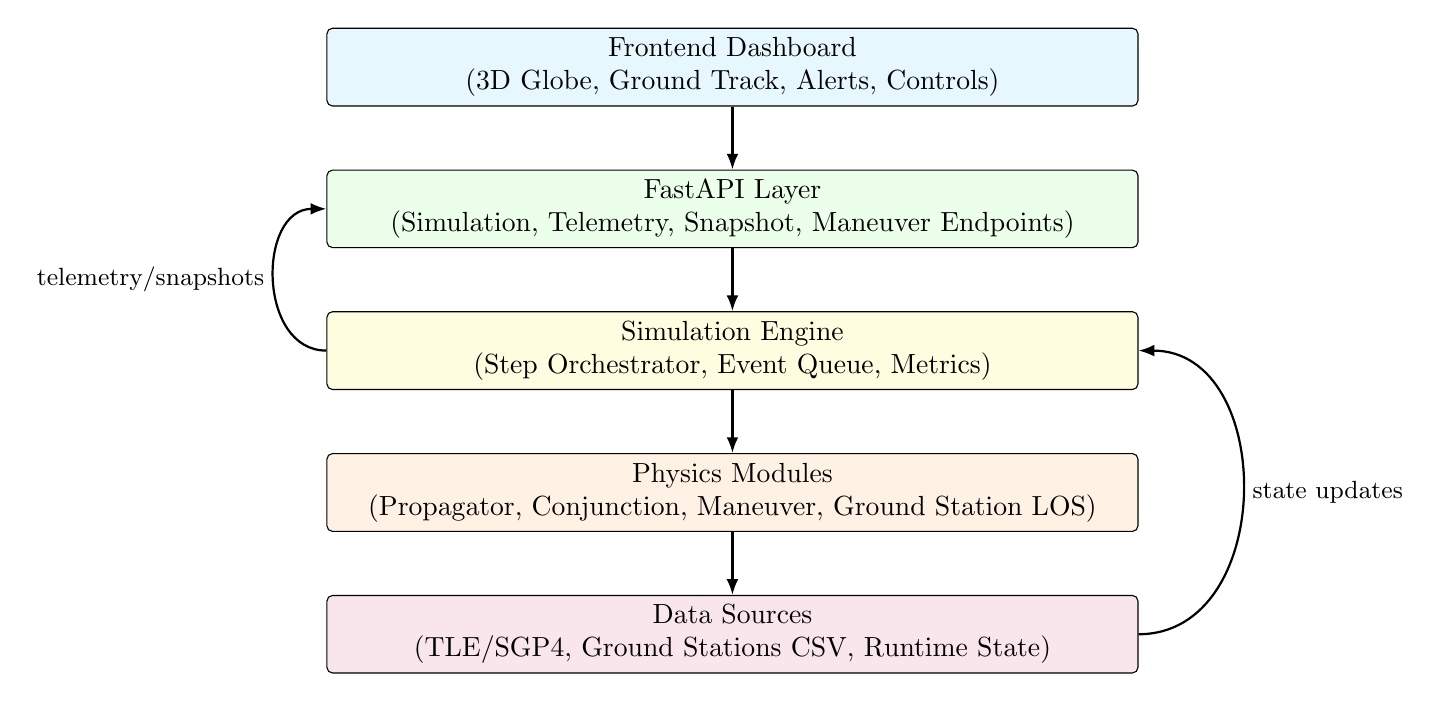
\begin{tikzpicture}[
  node distance=8mm,
  box/.style={draw, rounded corners=2pt, align=center, minimum width=10.3cm, minimum height=9mm, fill=blue!3},
  arr/.style={-{Latex[length=2mm]}, thick}
]
\node[box, fill=cyan!10] (ui) {Frontend Dashboard\\(3D Globe, Ground Track, Alerts, Controls)};
\node[box, below=of ui, fill=green!8] (api) {FastAPI Layer\\(Simulation, Telemetry, Snapshot, Maneuver Endpoints)};
\node[box, below=of api, fill=yellow!12] (engine) {Simulation Engine\\(Step Orchestrator, Event Queue, Metrics)};
\node[box, below=of engine, fill=orange!10] (physics) {Physics Modules\\(Propagator, Conjunction, Maneuver, Ground Station LOS)};
\node[box, below=of physics, fill=purple!10] (data) {Data Sources\\(TLE/SGP4, Ground Stations CSV, Runtime State)};

\draw[arr] (ui) -- (api);
\draw[arr] (api) -- (engine);
\draw[arr] (engine) -- (physics);
\draw[arr] (physics) -- (data);
\draw[arr] (data.east) to[out=0,in=0,looseness=1.25] node[right,align=left,font=\small]{state updates} (engine.east);
\draw[arr] (engine.west) to[out=180,in=180,looseness=1.25] node[left,align=right,font=\small]{telemetry/snapshots} (api.west);
\end{tikzpicture}
\caption{End-to-end architecture implemented by Team MindMatrix.}
\end{figure}

\subsection{Operational Workflow}
\begin{figure}[h!]
\centering
\resizebox{0.98\linewidth}{!}{%
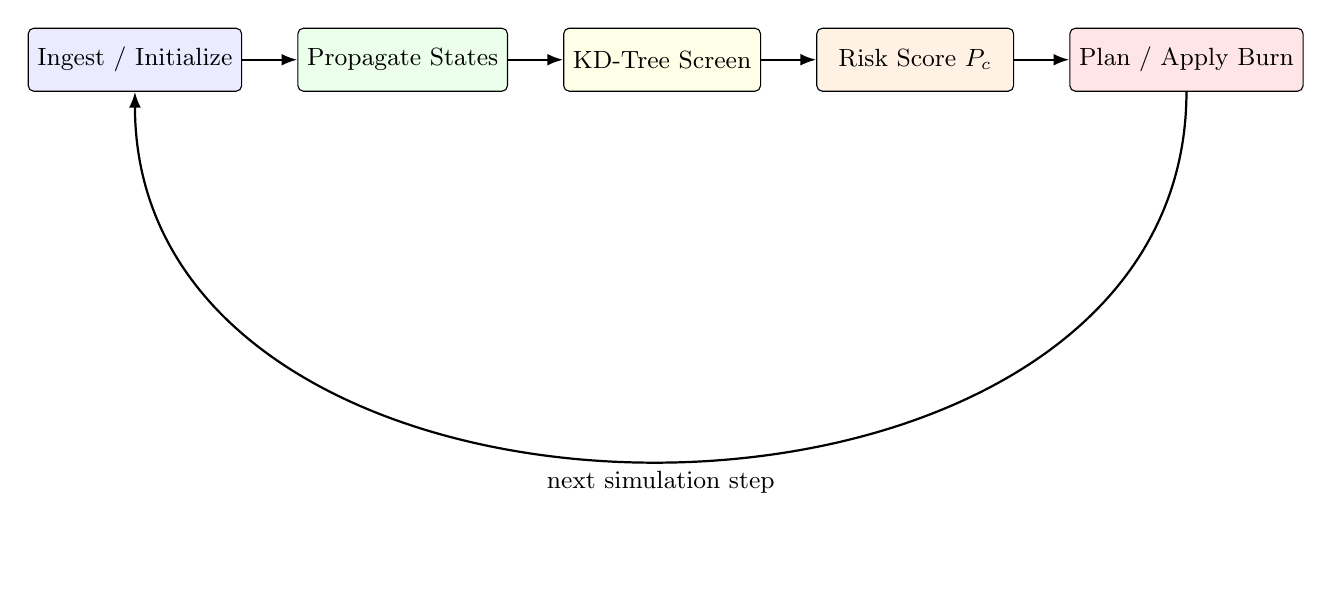
\begin{tikzpicture}[
  n/.style={draw, rounded corners=2pt, align=center, minimum width=2.5cm, minimum height=8mm, fill=gray!8, font=\small},
  arr/.style={-{Latex[length=2mm]}, thick}
]
\node[n, fill=blue!8] (a) {Ingest / Initialize};
\node[n, right=7mm of a, fill=green!8] (b) {Propagate States};
\node[n, right=7mm of b, fill=yellow!10] (c) {KD-Tree Screen};
\node[n, right=7mm of c, fill=orange!10] (d) {Risk Score $P_c$};
\node[n, right=7mm of d, fill=red!10] (e) {Plan / Apply Burn};

\draw[arr] (a) -- (b);
\draw[arr] (b) -- (c);
\draw[arr] (c) -- (d);
\draw[arr] (d) -- (e);
\draw[arr] (e.south) to[out=-90,in=-90,looseness=1.2] node[below,font=\small]{next simulation step} (a.south);
\end{tikzpicture}
}
\caption{Autonomous simulation-control loop.}
\end{figure}

\section{Implementation and Submission Notes}
\begin{itemize}
  \item API contract endpoints are implemented and tested: telemetry, maneuver scheduling, and simulation step.
  \item Frontend controls were hardened with queued stepping and guarded auto-run to prevent overlapping requests.
  \item Dockerized runtime is configured for port 8000 and deployment-ready launch.
\end{itemize}

\section{Conclusion}
Team MindMatrix's final system couples reliable numerical propagation with scalable spatial risk screening and constrained control planning in a clean service architecture. The resulting platform is both technically rigorous and operationally usable for live mission-style demonstrations.

\section*{Key Symbols}
\begin{center}
\begin{tabular}{ll}
\toprule
Symbol & Meaning \\
\midrule
$\mu$ & Earth gravitational parameter \\
$R_E$ & Earth equatorial radius \\
$J_2$ & second zonal harmonic coefficient \\
$P_c$ & collision probability \\
$d$ & miss distance \\
$I_{sp}$ & specific impulse \\
$g_0$ & standard gravity \\
\bottomrule
\end{tabular}
\end{center}

\end{document}
